\chapter{System Architecture}
\label{ch:architecture}

After the context in which the solution is settled has been described in \autoref{ch:basic-concepts}, \autoref{ch:requirements}
inspected Apache Flink and Apache Kafka according available sources of data and evaluated the data based on defined criteria
of data quality. As a result, the functional and non-functional requirements had been defined. According to the main goals of this thesis,
the collection of system and application data from Apache Flink and Apache Kafka and storage of collected data in a
centralized persistence system, the following sub-problems had been identified:

\begin{enumerate}
    \item Both source systems operate as distributed systems which consists of multiple instances of Apache
    Flink Job- and TaskManagers or Apache Kafka brokers, producers and consumers respectively. The software solution proposed
    must enable the collection of data from multiple application instances to gain an overall picture of the entire system.
    \item The process of data collection mustn't cause a negative impact on source systems. Since Apache Flink and Apache Kafka
    are both systems processing large amounts of data very fast, the utilization of system resources like cpu and memory of the
    collecting system must be kept as low as possible.
    \item As a result, the data must be transfered to the storage system with as less input/output operations and as fast
    as possible, to become available for possible data consumers immediately.
    \item The system architecture must provide a mechanism for the integration of possible data consumers which are unknown at
    the point of this thesis.
\end{enumerate}

The following chapter introduces the \textit{"Collector-Platform"} as a pipeline of data collection, transport and storage with the purpose
to collect data of distributed Apache Flink and Kafka systems and make it available for consumers that are potentially unknown at present
as fast as possible. The components will be discussed at architectural level, whereas implementation details follow in \autoref{ch:implementation}.

\section{The "Collector-Platform"}

According to the requirements in \autoref{ch:requirements}, the \textit{"Collector-Platform"} is responsible to perform the
following operations, which describe the pipeline the data in running throught on each source system. Irrespective of the source system,
the sequence remains the same for Apache Flink and Kafka or any other source system the \textit{CollectorClient} is installed on,
it just differs in the implementations of data collection:

\begin{figure}[H]
	\centering
	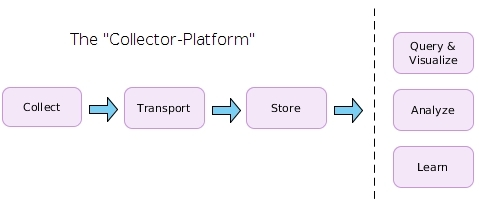
\includegraphics[width=0.8\textwidth]{../images/06-collect-pipeline.jpg}
	\caption{Collector Pipeline, \cite{VanL14}}
	\label{fig:colletor-pipeline}
\end{figure}

The the first step is the collection of data defined in \autoref{ch:requirements} on the Apache Flink and Apache Kafka source
systems. This includes collection of system data with the Dstat system utility as well as application specific data provided
by JMX or REST respectively. Once the the corresponding data had been retrieved and converted into a structured JSON format,
the data must leave source systems in the second step to reach the storage system at last, where they become available for
visualization tools, analytical processing or as a source for Machine Learning applications. \autoref{ch:evaluation} introduces
a sample application to demonstrate the possibilities for the integration of data consumers using the Stream Processing capabilities
of Apache Flink.

The "Collector-Platform" consist of the following components and will be discussed in the corresponding sections:

\begin{itemize}
    \item CollectorClient
    \item CollectorManager
    \item Consul ClientRegistry
    \item Kafka Message-Broker
    \item Logstash-Processor
    \item Elasticsearch Index
\end{itemize}

The following diagram shows an overview of all components involved and the interactions between them to fulfil the
requirements of data collection, transport and storage on the example of one Apache Flink JobManager and TaskManager as
source systems.

\begin{figure}[H]
	\centering
	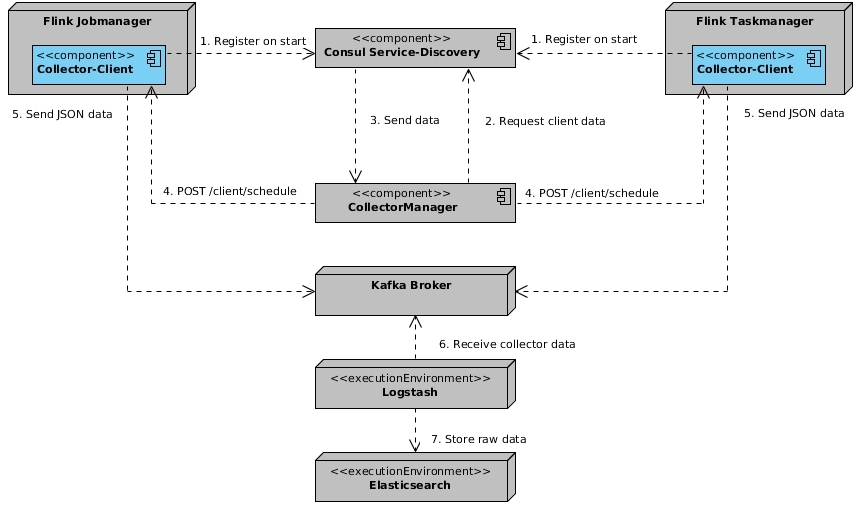
\includegraphics[width=1.0\textwidth]{../uml/component-diagram.jpg}
	\caption{The "Collector-Platform"}
	\label{fig:collector-platform}
\end{figure}

The \textit{CollectorClient}s installed on source systems, registers itself on application start with a central client registry, using
an unique identifier \verb|collector-client| \textbf{(1)}. This registry manages all registred clients and provides an interface
that allows the \textit{CollectorManager} to fetch network location (IP address and port) data for all clients that is required
to address the individual clients. The \textit{CollectorManager} uses this interface to display a list of all registred
\textit{CollectorClients} in a basic HTML user interface \textbf{(2,3)}. In addition, \textit{CollectorManager} fetches additional
meta information of the client \textbf{(4)}, like its host name and registered \textit{Collector}s, provided by the implementation
of the \textit{CollectorClient}.

In the next step, the process of data collection can be triggered using the \textit{CollectorManager}s user interface \textbf{(5)}.
Therefore, the \textit{CollectorManager} sends a HTTP \verb|POST| request with an appropriate JSON request body and receives a
status response that containing the status of the \textit{CollectorClient} that can be \verb|RUNNING| or \verb|STOPPED|,
according to the action that is triggered by the web user interface.

Now, the \textit{CollectorClient} is active and collects data corresponding the \textit{Collector} implementations registered in
the clients internal registry, see \autoref{sec:impl-collector-client}. Once all data of a single
\textit{Collector} implementation has been collected and transformed into a structured JSON format, the result will be enriched
with a client timestamp and the clients identification given by the IP address and the port the client is availabe at, and published to the
\textit{Kafka Message-Broker} \textbf{(6)}.

The \textit{Kafka Message-Broker} is the next step in the data pipeline and is the integration point for possible consumers
of data received by distributed \textit{CollectorClient}s. Due to the publish-subscribe principle Apache Kafka is based on,
potential consumers just need to subscribe to the \verb|collector-outbound-topic| for the data to become accessible.

The Logstash-Processor is the primary consumer of the data produced by \textit{CollectorClient}s. It receives outgoing \textit{CollectorClient}
data by subscribing to the \verb|collector-outbound-topic| topic, the clients publish the data into \textbf{(7)}. The Logstash-Processor performs
two essential tasks: it creates the required indexes for storing the data in Elasticserach and converts incoming data into an internal
message format that allows the data to be stored in Elasticsearch.

The Elasticsearch Index ist the last step in the \textit{"Collector-Platform"} \textbf{(8)}. It is the data sink where all collected data will be stored at.
The data is now available for querying or visualization.

For a deeper understanding, the following sections introduce the components and their corresponding functions described above.
Chosen frameworks and technologies will not be discussed in much detail, but it will be explained why each technology or
approach has been chosen.

\section{The "Collector" implementations}

This set of classes builds the core for collecting data on source systems and takes the responsibility for fetching
system data (\autoref{tbl:dstatcategories}) with the Dstat system tool as well as application data for Apache Flink
and Apache Kafka using the JMX interface (\autoref{tbl:jmxjvmdata}) and via REST for Apache Flink only
(\autoref{tbl:http-api-flink}). As shown in \autoref{ch:implementation}, all implementations are based on the
\textit{Collector} interface, what enables the handling of different realizations of data collection in a uniform way.

\section{CollectorClient}

The CollectorClient is main entry point for bringing data into the platform and belongs to the "Data" layer according to
\autoref{img:taxonomy-bigdata-applications}. It is a simple Java application and will have to be installed on source systems.
The module uses the concrete \textit{Collector} implementations described above, according to the source system and
depending on which \textit{Collector}s are registered in the client. The client contains and internal registration to enable
a mechanism to add or remove \verb|Collector| implementations without the need to change the implementation of the
\textit{CollectorClient}.

For the scheduling purposes of the collection process, the client provides a REST resource that enables the start and stop of data
collection from the HTML user interface provided by the \textit{CollectorManager} component.
This endpoint is available under the location \verb|http://{client-host}:{client-port}/client/schedule| and expects HTTP \verb|POST| requests
with a request body containing JSON data with an appropriate \textit{ScheduleRequest} for starting/stopping the data collection process.

Once started, the collection process that will be triggered by the client itself in a configurable interval, which is 5 seconds by default,
the resulted data will be send to an Apache Kafka topic called \verb|collector-outbound-topic|. The name of the topic explains the
purpose of the topic, it acts as the data sink for \textit{CollectorClient}s and separates the clients as the producing compontent
from data consumers.

Besides the scheduling REST resource, the client contains an endpoint \newline \verb|http://{client-host}:{client-port}/client/metadata|
that provides metatdata for the individual client and is required for displaying more detailed information about the client in the
\textit{CollectorManager}.

Corresponding to the \verb|Collector| implementations registered in an internal registry, the client creates a continous stream
of \verb|Collector| data, a stream of "immutable facts" concerning the the system and application state of the underlying source
system at a given point of time. Every data event created by the client contains the client's timestamp, the IP address and the port thus the
origin of the data can identified. Appendix A contains the full JSON results for all available \textit{Collector} implementations.

The client follows the approach to operate in a process that is separated to the JVM process the source system is running in.
To enable the \textit{CollectorClient}s to access to the management interfaces introduced in \autoref{tbl:jmxjvmdata} on the remote JVM
of Apache Flink and Apache Kafka, the source system must to be configured to allow the connection from a remote JMX client. \autoref{ch:evaluation}
explains the adjustments that had been made on the example of Apache Flink. This in turn brings the disadvantage of potential
security risks that occur by allowing remote connections on a given port.

An alternative would have been to use the capabilities of dynamic bytecode intrumentation provided by the core of Java. Because
Apache Flink and Apache Kafka both are based on the JVM, it would have been possible to instrument the Flink or Kafka process itself,
to perform the data collection in the same process. This approach was not pursued in this thesis, because the instrumentation causes
a performance impact, that can be avoided by separation of collection in an individual process.

\section{CollectorManager}
\label{sec:arch-collector-manager}
Due to the fact that Apache Flink and Apache Kafka are composed of several interacting components and thus building
a distributed system, the \textit{"Collector-Platform"} builds a distributed system as well. Based on the requirement to provide a
mechanism to schedule the collection process in distributed \textit{CollectorClient}s, the \textit{CollectorManager} represents the management
component for the distributed system of clients by providing an overview of registered clients in the platform and
the possibility to start/stop individual clients using an HTML based user interface.

\begin{figure}[H]
 	\centering
 	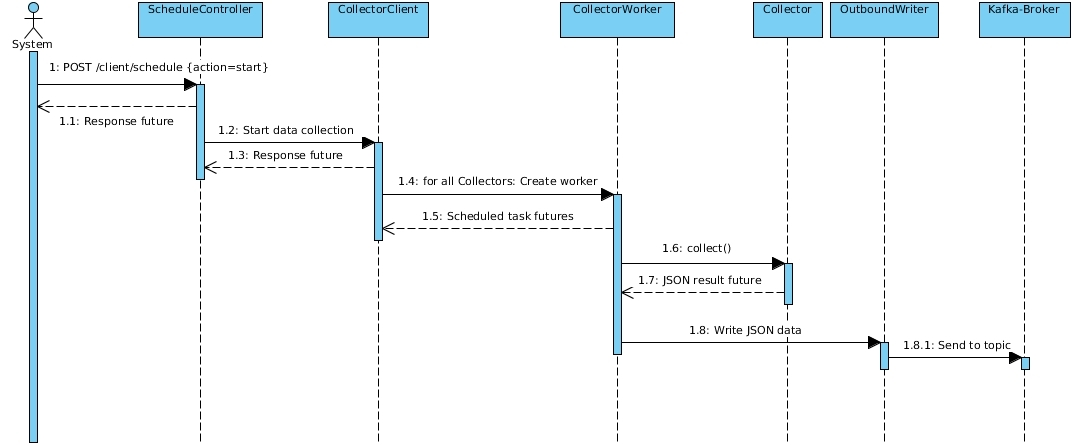
\includegraphics[width=1.0\textwidth]{../uml/sequence-scheduling.jpg}
 	\caption{Sequence diagram 'Client scheduling'}
 	\label{fig:sequence-client-scheduling}
 \end{figure}

The sequence diagram above presents the process of starting an individual \textit{CollectorClient}. The client receives a HTTP
\verb|POST| request that contains an appropriate \textit{ScheduleRequest} for starting the client. If the request is syntactically
correct, the client starts data collection as discussed above.

\section{Consul Client-Registry}

The \textit{Client-Registry} is a dedicated web service and acts as a central registry for all \textit{CollectorClient} instances
in the platform and makes the information about registered clients available for the \textit{CollectorManager}.
For the realization of a public registry for distributed clients, the platform uses Consul, a service-registry, that enables the discovery
of web services based on unique identifiers instead of host address and port information. Since the \textit{CollectorClient} is a web service itself,
clients register with the service name \verb|collector-client| when the client application is started. The \textit{CollectorManager}
queries the Consul node for existing instances of services named \verb|collector-client| which results in a list of registred client instances,
that contains the required information like host and port for using the scheduling and metadata endpoints in the managers user interface.

\begin{figure}[H]
	\centering
	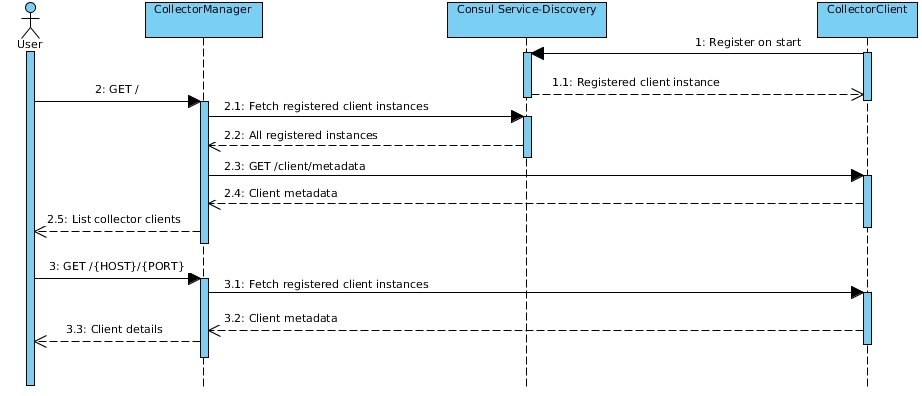
\includegraphics[width=1.0\textwidth]{../uml/sequence-discovery.jpg}
	\caption{Sequence diagram 'Client discovery'}
	\label{fig:sequence-client-discovery}
\end{figure}

Using an central registry instance for discovering \textit{CollectorClient} instances decouples the \textit{CollectorManager} from the
need to know detailed client information required for the localization of the service. Due to the fact that
client addresses and ports are dynamically assigned and may change in distributed cloud environments, the service registry provides
a scalable and flexible way to discover the providers of a given service name, \verb|collector-client| in this case.

\section{Kafka Message-Broker}

The \textit{Kafka Message-Broker} integrates distributed \textit{CollectorClient}s to an overall system by providing a
message queue for transporting data from clients to the \textit{Logstash-Processor}. The \textit{CollectorClient}s can publish
its data to the queue and the other applications can asynchronously read it from the queue at any time.
The usage of Apache Kafka as a publish-subscribe queuing service allows a separation of \textit{CollectorClient}s as publishers and the
\textit{Logstash-Processor} and other potential as subcribers by buffering messages between stream producing and consuming systems.

\section{Logstash-Processor}
The \textit{Logstash-Processor} receives the messages that arrive in the \verb|collector-outbound-topic|. Although is is often thougth that
Logstash is only capable of processing log files, it is more a data pipeline that enable the processing and transformation of log and other
event data from a variety of systems. According to this thesis, it receives custom JSON data from clients and creates the indexes
for storing the received JSON data in the \textit{Elasticsearch Index}.

\section{Elasticsearch Index}

Elasticsearch is distributed, scalable, and highly available full-text search engine based on the Apache Lucene search index.
It provides an HTTP web interface for managing, storing and quering schema-free JSON documents and is a widely used storage system
of Big Data Analytics Applications. The search engine, the Logstash-Indexer and the Kibana visualization tool in combination are
often refered to as "ELK" and provides a an end-to-end stack for central data collection and analysis as well as a graphical
presentation of raw and analyzed data.

Elasticsearch allows the storage of collected data in its raw JSON format, what was a decisive criterion in the process of choosing an
appropriate database for the \textit{"Collector-Platform"}. Due to the fact that potential consumers of data produced by \textit{CollectorClient}s
are unknown at the time of the thesis, the JSON format provides an universal structure that can be processed by any application.

\section{Summary}

This chapter introduced the \textit{"Collector-Platform"} as data pipeline for collecting and storing system and application data
on Apache Flink and Apache source systems. The pipeline starts on the \textit{CollectorClient} instances, small web services that need
to be installed on source systems, the data that will be collected depends on the \verb|Collector| implementations registered
in the client. Each \verb|Collector| implementation produces its own custom result formatted in JSON that will be published to a
\textit{Kafka Message-Broker}. The broker provides a data queue that decouples data producers and consumers. Moreover using
a queing system prevents the requirement of specialized operations for exchanging data and helps to decrease the performance impact on
Apache Flink and Apache Kafka source systems.

The \textit{Logstash-Processor} is a subcriber to the \verb|collector-outbound-topic|, thus it receives
collected data, creates required indexes and transforms the data to be stored in Elasticsearch.

To enable the scheduling of the data collection process, the \textit{CollectorManager} provides an access point to start and stop
\textit{CollectorClients} using a REST resource available for each client. The REST paradigma, discussed in \autoref{sec:rest} provides
an uniform interface for machine-to-machine communication and the exchange of data
between participants in a distributed software system based on the existing HTTP infrastructure.

A centralized \textit{Consul Client-Registry} as mechanism to discover \textit{CollectorClient}s independently of concrete network locations
has been discussed in the context of the platform.

Whereas this chapter just introduced an architectural overview of the components involved, the next \autoref{ch:implementation} discusses
details of the implementation and the technologies used for the realization of the \textit{Collector-Platform}.